\section{1174086 - Tia Nur Candida}
\subsection{Teori}
\begin{enumerate}
	\item Kenapa file suara harus di lakukan MFCC. dilengkapi dengan ilustrasi atau gambar.
	\hfill\break
	Mampu untuk menangkap karakteristik suara yang sangat penting bagi pengenalan suara, atau dengan kata lain dapat menangkap informasi-informasi penting yang terkandung dalam signal suara. Menghasilkan data seminimal mungkin, tanpa menghilangkan informasi-informasi penting yang dikandungnya. Mereplikasi organ pendengaran manusia dalam melakukan persepsi terhadap signal suara.
	\begin{figure}[H]
		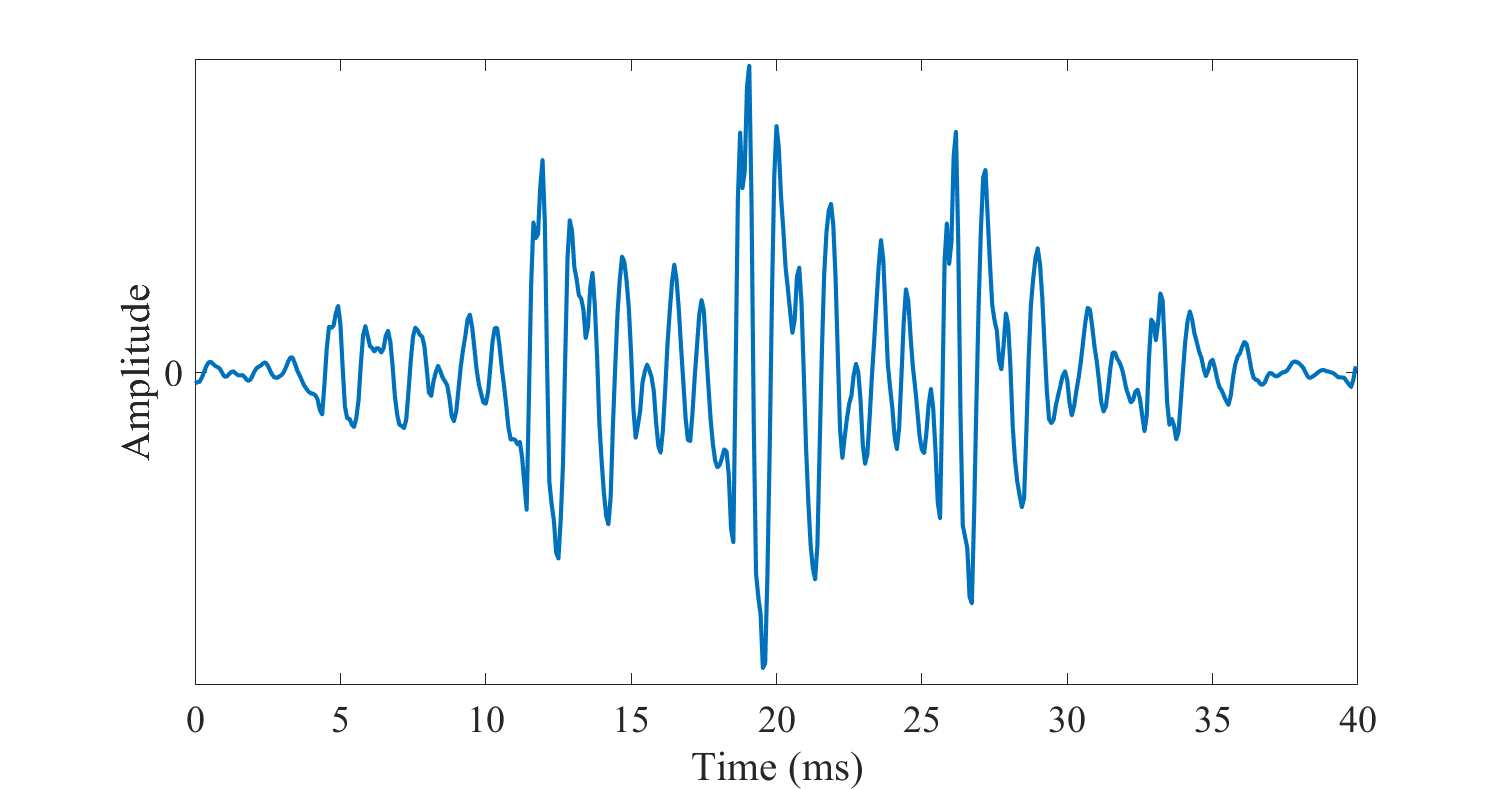
\includegraphics[width=4cm]{figures/1174086/6/7.png}
		\centering
		\caption{MFCC}
	\end{figure}
	
	
	\item Konsep dasar neural network dilengkapi dengan ilustrasi atau gambar
	\hfill\break
	Neural Network ini terinspirasi dari jaringan saraf otak manusia. Dimana setiap neuron terhubung ke setiap neuron di lapisan berikutnya. Lapisan pertama menerima input dan lapisan terakhir memberikan keluaran. Struktur jaringan, yang berarti jumlah neuron dan koneksinya, diputuskan sebelumnya dan tidak dapat berubah, setidaknya tidak selama training. Juga, setiap input harus memiliki jumlah nilai yang sama. Ini berarti bahwa gambar, misalnya, mungkin perlu diubah ukurannya agar sesuai dengan jumlah neuron input.
	\begin{figure}[H]
		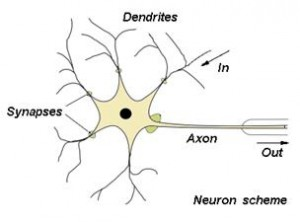
\includegraphics[width=4cm]{figures/1174086/6/8.jpg}
		\centering
		\caption{Contoh Pembobotan Neural Network}
	\end{figure}

	\item Konsep pembobotan dalam neural network. dilengkapi dengan ilustrasi atau gambar
	\hfill\break
	Bobot mewakili kekuatan koneksi antar unit. Jika bobot dari node 1 ke node 2 memiliki besaran lebih besar, itu berarti bahwa neuron 1 memiliki pengaruh lebih besar terhadap neuron. 2. Bobot penting untuk nilai input. Bobot mendekati nol berarti mengubah input ini tidak akan mengubah output. Bobot negatif berarti meningkatkan input ini akan mengurangi output. Bobot menentukan seberapa besar pengaruh input terhadap output. Seperti contoh berikut :
	\begin{figure}[H]
		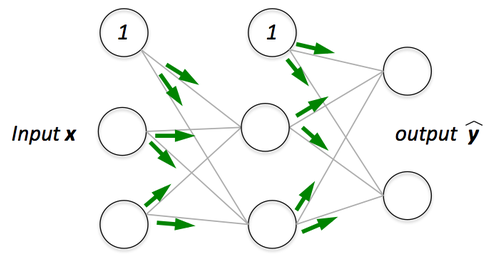
\includegraphics[width=4cm]{figures/1174086/6/2.png}
		\centering
		\caption{Contoh Pembobotan Neural Network}
	\end{figure}

	\item Konsep fungsi aktifasi dalam neural network. dilengkapi dengan ilustrasi atau gambar
	\hfill\break
	Fungsi aktivasi digunakan untuk memperkenalkan non-linearitas ke jaringan saraf. Ini menekan nilai dalam rentang yang lebih kecil yaitu. fungsi aktivasi Sigmoid memeras nilai antara rentang 0 hingga 1. Ada banyak fungsi aktivasi yang digunakan dalam industri pembelajaran yang dalam dan ReLU, SeLU dan TanH lebih disukai daripada fungsi aktivasi sigmoid. Ilustrasinya, ketika fungsi aktivasi linier, jaringan saraf dua lapis mampu mendekati hampir semua fungsi. Namun, jika fungsi aktivasi identik dengan fungsi aktivasi F (X) = X), properti ini tidak puas, dan jika MLP menggunakan fungsi aktivasi yang sama, seluruh jaringan setara dengan jaringan saraf lapis tunggal.

	\item Cara membaca hasil plot dari MFCC,dilengkapi dengan ilustrasi atau gambar
	\hfill\break
	Berikut merupakan hasil plot dari rekaman suara :
	\begin{figure}[H]
		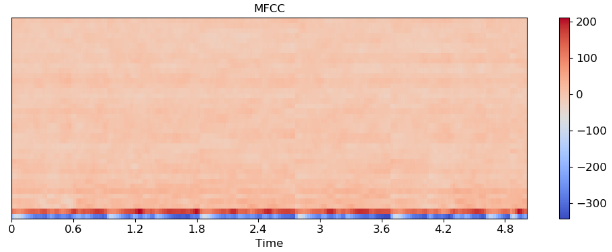
\includegraphics[width=4cm]{figures/1174086/6/1.png}
		\centering
		\caption{Cara Membaca Hasil Plot MFCC}
	\end{figure}
	Dari gambar tersebut dapat diketahui :
	\begin{itemize}
		\item Terdapat 2 dimensi yaitu x sebagai waktu, dan y sebagai power atau desibel.
		\item Dapat dilihat bahwa jika berwarna biru maka power dari suara tersebut rendah, dan jika merah power dari suara tersebut tinggi
		\item Dibagian atas terdapat warna merah pudar yang menandakan bahwa tidak ada suara sama sekali dalam jangkauan tersebut.
	\end{itemize}
	
	\item Jelaskan apa itu one-hot encoding,dilengkapi dengan ilustrasi kode dan atau gambar.
	\hfill\break
	One-hot encoding adalah representasi variabel kategorikal sebagai vektor biner. Mengharuskan nilai kategorikal dipetakan ke nilai integer. Kemudian, setiap nilai integer direpresentasikan sebagai vektor biner yang semuanya bernilai nol kecuali indeks integer, yang ditandai dengan 1.
	\begin{figure}[H]
		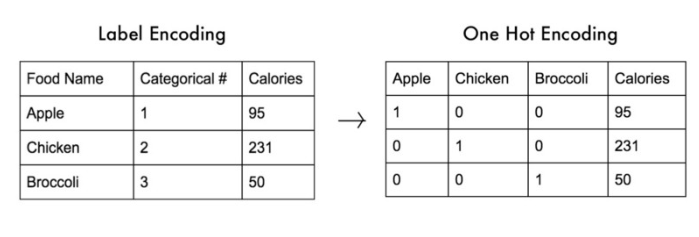
\includegraphics[width=4cm]{figures/1174086/6/3.png}
		\centering
		\caption{One Hot Encoding}
	\end{figure}

	\item Fungsi dari np/.unique dan to categorical dalam kode program,dilengkapi dengan ilustrasi atau gambar.
	\hfill\break
	Untuk np unique fungsinya yaitu menemukan elemen unik array. Mengembalikan elemen unik array yang diurutkan. Ada tiga output opsional selain elemen unik:\\
	\begin{itemize}
		\item Indeks array input yang memberikan nilai unik
		\item Indeks array unik yang merekonstruksi array input
		\item Berapa kali setiap nilai unik muncul dalam array input.
	\end{itemize}
	\begin{figure}[H]
		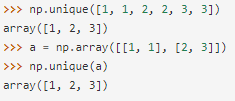
\includegraphics[width=4cm]{figures/1174086/6/4.png}
		\centering
		\caption{Numpy Unique}
	\end{figure}

	Untuk  To Categorical fungsinya untuk mengubah vektor kelas (integer) ke matriks kelas biner.
	\begin{figure}[H]
		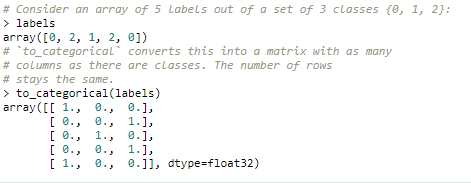
\includegraphics[width=4cm]{figures/1174086/6/5.png}
		\centering
		\caption{To Categorical}
	\end{figure}

	\item Fungsi dari Sequential dalam kode program,dilengkapi dengan ilustrasi atau gambar.
	\hfill\break
	Sequential berfungsi sebagai tumpukan linear lapisan. COntohnya sebagai berikut :
	\begin{figure}[H]
		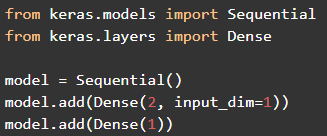
\includegraphics[width=4cm]{figures/1174086/6/6.png}
		\centering
		\caption{Sequential}
	\end{figure}

\end{enumerate}
\subsection{Praktek}
\begin{enumerate}
	\item Penjelasan isi data GTZAN Genre Collection dan data dari Freesound.
	\lstinputlisting[firstline=9, lastline=28]{src/1174086/6/1174086.py}

	\item Penjelasan perbaris kode program dari display MFCC.
	\lstinputlisting[firstline=30, lastline=40]{src/1174086/6/1174086.py}

	\item Penjelasan perbaris code dari Extract Feature Song.
	\lstinputlisting[firstline=43, lastline=51]{src/1174086/6/1174086.py}

	\item Penjelasan perbaris code dari Generate Features and Labels.
	\lstinputlisting[firstline=55, lastline=72]{src/1174086/6/1174086.py}

	\item Penjelasan penggunaan fungsi Generate Features and Labels sangat lama ketika Meload Dataset Genre.
	\lstinputlisting[firstline=76, lastline=78]{src/1174086/6/1174086.py}

	\item Kenapa harus dilakukan pemisahan data training dan dataset sebesar 80\%
	\lstinputlisting[firstline=80, lastline=92]{src/1174086/6/1174086.py}

	\item Parameter dari fungsi Sequensial().
	\lstinputlisting[firstline=95, lastline=100]{src/1174086/6/1174086.py}

	\item Parameter dari fungsi Compile().
	\lstinputlisting[firstline=102, lastline=105]{src/1174086/6/1174086.py}

	\item Parameter dari fungsi Fit().
	\lstinputlisting[firstline=107, lastline=108]{src/1174086/6/1174086.py}

	\item Parameter dari fungsi Evaluate().
	\lstinputlisting[firstline=110, lastline=112]{src/1174086/6/1174086.py}

	\item Parameter dari fungsi Predict().
	\lstinputlisting[firstline=115, lastline=115]{src/1174086/6/1174086.py}

\end{enumerate}
\subsection{Penanganan Error}
\begin{enumerate}
	\item SS Error
	\begin{figure}[H]
		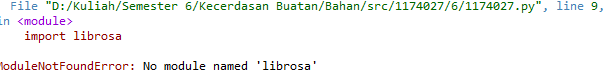
\includegraphics[width=4cm]{figures/1174086/error/6_no_module.png}
		\centering
		\caption{No Module Name error}
	\end{figure}
	\item Jenis Error
	\begin{itemize}
		\item No Module
	\end{itemize}
	\item Cara Penanganan
	\hfill\break
	Dengan cara melakukan instalasi module yang bersangkutan / menginstal library yang digunakan
\end{enumerate}
\subsection{Bukti Tidak Plagiat}
\begin{figure}[H]
    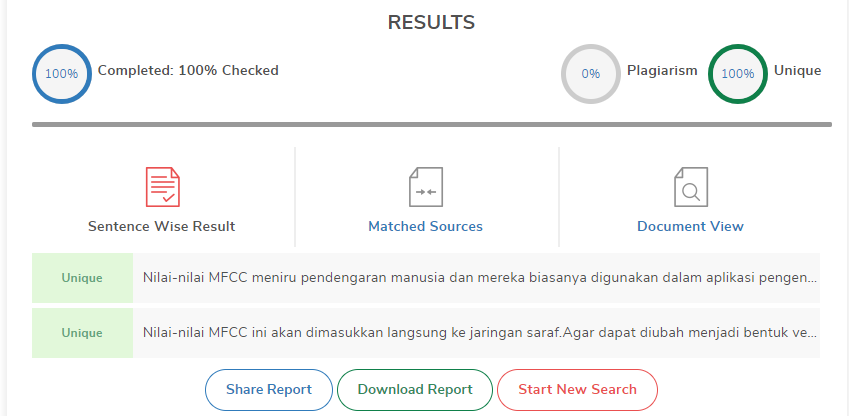
\includegraphics[width=4cm]{figures/1174086/bukti/6.png}
    \centering
    \caption{Tidak Melakukan Plagiat Pada Ch 6}
\end{figure}
